\section{White Rabbit} \label{sec:wr}

\acrfull{wr} hace referencia tanto al protocolo diseñado como mejora de 
\gls{ptp}v2 como al proyecto internacional que se encarga de su desarrollo y 
mantenimiento. Inicialmente parte como una tecnología desarrollada por el 
\gls{cern} para actualizar el sistema de sincronización y envío de datos de 
control para su complejo de aceleradores de partículas. Gracias a el espíritu 
abierto con el que se desarrolló la tecnología (y a su prometedor rendimiento) 
fueron sumándose otras instituciones al desarrollo, tanto desde el ámbito 
académico, donde cabe destacar el Centro de Investigación de Iones Pesados 
(\textit{Gesellschaft für Schwerionenforschung}, GSI en alemán) en Alemania o 
la propia Universidad de Granada; como desde el empresarial, donde se está 
intentando expandir la tecnología al ámbito industrial. Ejemplos de ello son la 
empresa Seven Solutions (\text{spin-off} de la UGR) en Granada, o CreoTECH en 
Polonia. 

Aunque el empuje en el ámbito de la ciencia es mucho más 
evidente gracias a la inclusión de \textit{WR} en instalaciones para 
aceleradores de partículas, institutos metrológicos o en sistemas de 
adquisición ditribuida como el caso del proyecto Square Kilometre Array (SKA) 
que se está contruyendo en Sudáfrica y que una vez concluido será el 
instrumento de observación astronómica más sensible jamás construido por la 
humanidad. En el caso de la empresa privada, \gls{wr} se ve todavía como una 
tecnología muy prometedora para diversas áreas como Smart Grid, 
Geo-posicionamiento o para las telecomunicaciones, que aún necesita madurar. 
Esto está a punto de cambiar gracias a su inclusión en la próxima revisión del 
estándar \gls{ptp} bajo un nuevo perfil de alta precisión.

Los objetivos de desarrollo iniciales estaban enfocados al entorno de los 
aceleradores de partículas, priorizando una sincronización de calidad junto a 
un sistema que fuese determinista y fácil de mantener:

\begin{itemize}
	\item Lograr para una red de miles de nodos, conectados por enlaces de 
	fibra óptica de hasta 10 km, una diferencia menor del nanosegundo entre dos 
	nodos cualesquiera de la red, es decir, una exactitud de sincronización 
	\textbf{sub-nanosegundo}. Además, se requiere una precisión en el orden del 
	picosegundo.
	
	\item Permitir que el enlace utilizado para los paquetes del protocolo 
	\gls{wr} se pueda \textbf{compartir para} el envío de \textbf{datos de 
	propósito general}, 
	reduciéndo así costes en el despliegue de las infraestructuras.
	
	\item Realizar un desarrollo \textbf{simple y escalable} que no necesite de 
	sofisticados procedimientos de configuración o calibración.
	
	\item Establecer un envío \textbf{determinista} para los paquetes 
	prioritarios, con 
	retardos que no superen ciertos valores umbrales. Esto es especialmente 
	importante en sistemas de control donde la respuesta a un evento no puede 
	exceder un tiempo límite en su envío.
	
	\item Proveer un \textbf{diseño} de referencia \textbf{abierto} a la 
	comunidad 
	(tanto \textit{hardware} como \textit{software}) para fomentar el 
	desarrollo por parte de esta, y evitar las ligaduras con fabricantes.
\end{itemize}

En la actualidad se puede afirmar que en su mayor parte se han cumplido dichos 
objetivos. El requisito principal de rendimiento es algo que se ha conseguido 
en su mayor parte aunque hace falta aportar datos acerca del comportamiento del 
protocolo en redes realmente grandes con un gran número de nodos. La tendencia 
actual en cuanto a rendimiento se centra en la mejora de la exactitud alcanzada 
en escenarios no tan típicos, como enlaces de larga distancia o escenarios con 
cambios en las condiciones de operación. También se investiga como reducir el 
ruido producido por los componentes del sistema de sincronización para lograr 
una precisión en el orden del femtosegundo. El envío determinista es algo que 
no siempre se logra, ya que se puede producir la pérdida de algún paquete de 
alta prioridad en casos de congestión del enlace. Las herramientas de gestión y 
mantenimiento es otro punto al que todavía le queda trabajo por delante y al 
que se está prestando bastante atención dado que son algo crucial si se 
pretende extender el uso del protocolo más allá del ámbito científico.

El protocolo \gls{wr} fue diseñado como una extensión del protocolo IEEE 
1588-2008 (\gls{ptp}v2) al que se añadieron varias mejoras como un modelo de 
enlace más preciso, técnicas de calibración automática o sintonización de los 
relojes mediante el envío de la frecuencia maestra codificada en los paquetes 
transmitidos.

\begin{figure}
	\centering
	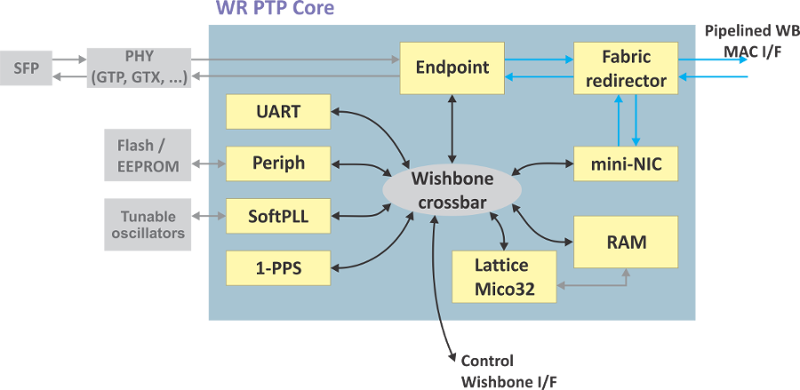
\includegraphics[width=0.7\linewidth]{imagenes/wrpc_inside}
	\caption[Esquema de bloques del WR PTP Core]{En este esquema de bloques se 
	incluyen los componentes principales que componen la arquitectura del WR 
	PTP Core. El bloque principal hace referencia a los componentes en la parte 
	de lógica repogramable, mientras que fuera se incluyen componentes que o 
	bien se incluyen como soporte hw dentro de la FPGA (PHY) o bien son 
	componentes externos que se conectana a algún pin para comunicarse con los 
	elementos internos. Imagen tomada de \cite{Daniluk2012}.}
	\label{fig:wrpcinside}
\end{figure}

\incomment{echar mas leña al fuego}




